%% ****** Start of file apstemplate.tex ****** 
%%
%%
%%   This file is part of the APS files in the REVTeX 4.2 distribution.
%%   Version 4.2a of REVTeX, January, 2015
%%
%%
%%   Copyright (c) 2015 The American Physical Society.
%%
%%   See the REVTeX 4 README file for restrictions and more information.
%%
%
% This is a template for producing manuscripts for use with REVTEX 4.2
% Copy this file to another name and then work on that file.
% That way, you always have this original template file to use.
%
% Group addresses by affiliation; use superscriptaddress for long
% author lists, or if there are many overlapping affiliations.
% For Phys. Rev. appearance, change preprint to twocolumn.
% Choose pra, prb, prc, prd, pre, prl, prstab, prstper, or rmp for journal
%  Add 'draft' option to mark overfull boxes with black boxes
%  Add 'showkeys' option to make keywords appear
%\documentclass[aps,prl,preprint,groupedaddress]{revtex4-2}
\documentclass[aps,prl,reprint,superscriptaddress,showkeys]{revtex4-2}
%\documentclass[aps,prl,reprint,groupedaddress]{revtex4-2}

\usepackage{amsmath, amsthm, amssymb}
\usepackage{graphicx}
\usepackage{subfigure}
\usepackage{wrapfig}
\usepackage{color}
\usepackage{bm}

% You should use BibTeX and apsrev.bst for references
% Choosing a journal automatically selects the correct APS
% BibTeX style file (bst file), so only uncomment the line
% below if necessary.
\bibliographystyle{apsrev4-2}

\begin{document}

% Use the \preprint command to place your local institutional report
% number in the upper righthand corner of the title page in preprint mode.
% Multiple \preprint commands are allowed.
% Use the 'preprintnumbers' class option to override journal defaults
% to display numbers if necessary
%\preprint{}

%Title of paper
\title{Estudio de especies reactivas de oxígeno producidas por nanopartículas de MnFe$_2$O$_4$ mediante espectroscopía EPR combinada con \textit{spin trapping}}

% repeat the \author .. \affiliation  etc. as needed
% \email, \thanks, \homepage, \altaffiliation all apply to the current
% author. Explanatory text should go in the []'s, actual e-mail
% address or url should go in the {}'s for \email and \homepage.
% Please use the appropriate macro foreach each type of information

% \affiliation command applies to all authors since the last
% \affiliation command. The \affiliation command should follow the
% other information
% \affiliation can be followed by \email, \homepage, \thanks as well.
\author{Ignacio Lembo Ferrari}
%\email[]{ignacio.lembo@ib.edu.ar}
%\homepage[]{Your web page}
%\altaffiliation{}
\affiliation{Instituto Balseiro}

%Collaboration name if desired (requires use of superscriptaddress
%option in \documentclass). \noaffiliation is required (may also be
%used with the \author command).
%\collaboration can be followed by \email, \homepage, \thanks as well.
%\noaffiliation
%\collaboration{Resonancias Magnéticas}


\date{\today}

\begin{abstract}
Se estudió la capacidad de las nanopartículas de MnFe$_2$O$_4$ para promover especies reactivas de oxígeno (ROS) en presencia de H$_2$O$_2$ mediante espectroscopía EPR junto con la técnica de \textit{spin trapping} para detectar los radicales formados. Se empleó el compuesto 5,5-Dimetil-1-pirrolina N-oxido (DMPO) como \textit{spin trap}. Se realizaron mediciones a los 10 y 40 minutos de inicio de la producción de ROS y se identificó la presencia de radicales hidroxilo a los 10 minutos, así como radicales hidroxilo y metilo a los 40 minutos. Utilizando un modelo de interacción Zeeman e hiperfina se describieron satisfactoriamente los espectros observados destacando la capacidad de esta técnica para caracterizar las ROS producidas por las nanopartículas de MnFe$_2$O$_4$.

\end{abstract}

% insert suggested keywords - APS authors don't need to do this
\keywords{EPR, Nanopartículas, ROS}

%\maketitle must follow title, authors, abstract, and keywords
\maketitle

% body of paper here - Use proper section commands
% References should be done using the \cite, \ref, and \label commands
% Put \label in argument of \section for cross-referencing
%\section{\label{}} 
\section{Introducción}

Las especies reactivas de oxígeno (ROS, por sus siglas en inglés) son especies altamente reactivas derivadas del oxígeno que se generan como subproducto natural del metabolismo oxidativo celular \cite{liu_biomedical_2020}. El anión superóxido $\cdot$O$_2^-$, el oxhidrilo $\cdot$OH (radiciales libres) y el peróxido de hidrógeno H$_2$O$_2$ son ejemplos de ROS. En concentraciones normales, las ROS son esenciales para el metabolismo fisiológico, regulan la respuesta celular a la hipoxia y la resistencia a agentes infecciosos y participan en varios sistemas de comunicación celular. No obstante, un desbalance en el equilibrio entre la producción de ROS y antioxidantes puede ocasionar daños en proteínas, ADN y estrés oxidativo el cual se ha relacionado con diversas enfermedades como cáncer, diabetes o enfermedades neurodegenerativas \cite{liu_biomedical_2020}. 

Trabajos recientes \cite{maldonado_actividad_nodate,gao_intrinsic_2007} han mostrado que existen nanopartículas de ferritas (MeFe$_2$O$_4$ donde Me es un metal con valencia 2) con la capacidad de catalizar la producción de ROS en presencia de H$_2$O$_2$ mediante una reacción en la superficie de las mismas. Este tipo de reacciones son catalizadas por un metal de transición, en este caso, el metal Me presente en la nanopartícula, y son conocidas como reacciones de Fenton \cite{FentonLXXIIIOxidationOT}

 \begin{equation}
    \text{Mn}^{2+} + \text{H}_2\text{O}_2 \longrightarrow \text{Mn}^{3+}  + \cdot ~ \text{OH} + \text{OH}^{-},
\end{equation}
\begin{equation}
    \text{Mn}^{3+} + \text{H}_2\text{O}_2 \longrightarrow \text{Mn}^{2+}  + \cdot ~ \text{OOH} + \text{H}^{+}.
\end{equation}

Los radicales libres son moléculas que poseen al menos un electrón desapareado, son altamente inestables y de naturaleza paramagnética. Actualmente, la espectroscopía por resonancia paramagnética electrónica (EPR) es la técnica más precisa para la detección de radicales libres. No obstante, debido a que el tiempo de vida media de los radicales es muy corto (del orden de 1 $\mu$s), no es posible detectarlos directamente mediante espectroscopía EPR. Para poder extender dicho tiempo de vida media se utiliza una técnica conocida como \textit{spin trapping}. Esta técnica consiste en añadir una molécula (\textit{spin trap}) a la muestra en estudio, la cual se combina con los radicales libres fomando una especie más estable conocida como aducto. Esto permite la detección y caracterización indirecta de los radicales formados en la muestra. En este trabajo se utilizó como \textit{spin trap} 5,5-Dimetil-1-pirrolina N-oxido (DMPO). Es importante destacar que los aductos formados radical-DMPO, además de detectar la presencia de radicales libres producidos, permite identificarlos. 

Combinando técnicas de medición y clasificación de radicales libres junto con aplicación de nanopartículas magnéticas se puede optimizar la producción de ROS en el organismo, lo cual potencialmente se puede utilizar para producir muerte celular en terapias oncológicas, disminuir efectos dañinos en MRI o intervenciones oftalmológicas \cite{zhou_reactive_2016, abdal_dayem_role_2017}. En este trabajo se estudiaron las especies radicales producidas a los 10 y 40 minutos de agregar H$_2$O$_2$ en una muestra de nanopartículas de MnFe$_2$O$_4$.


\section{Marco teórico \label{sec:teoriaEPR}}

Dado que el objeto de estudio son moléculas con un electrón desapareado que interactúan fuertemente con el entorno molécular. Se detallarán dichas interacciones en general y luego se analizará el caso particular de los aductos de radical-DMPO.

\subsection{Interacciones Zeeman e Hiperfina \label{sec:interacciones}}
Sea un sistema formado por un espín electrónico ($\mathbf{\hat{S}}$) y un espín nuclear ($\mathbf{\hat{I}}$) en un campo magnético $\mathbf{B_0}$, el hamiltoniano que describe esta interacción es \cite{weil_electron_2007}
\begin{equation}
    \mathcal{H} = g \mu_B ~ \mathbf{B_0} \cdot \mathbf{\hat{S}} + g_N \mu_N ~\mathbf{B_0} \cdot \mathbf{\hat{I}},
    \label{ec:Hzeeman}
\end{equation}
donde $g$ y $g_N$ son los factores de Landé asociados al electrón y al núcleo respectivamente, $\mu_B$ es el magnetón de Bohr y $\mu_N$ el magnetón nuclear. Este término se conoce como interacción Zeeman. Si además se considera la interacción de este espín electrónico con los espines nucleares vecinos, se debe adicionar al hamiltoniano de la Ec. (\ref*{ec:Hzeeman}) un término de interacción hiperfina que describa el acople entre espines electrónicos y nucleares. El hamiltoniano entonces queda
\begin{equation}
    \mathcal{\hat{H}} = g \mu_B ~\mathbf{B_0} \cdot \mathbf{\hat{S}} + g_N \mu_N ~\mathbf{B_0} \cdot \mathbf{\hat{I}} + \sum_{i=1}^{N} A_i~ \mathbf{\hat{S}} \cdot \mathbf{\hat{I}}_i,
    \label{ec:Hcompleto}
\end{equation}
donde $A_i$ es la constante hiperfina correspondiente al núcleo $i$. Despreciando el término de Zeeman nuclear en el hamiltoniano de la Ec. (\ref*{ec:Hcompleto}) debido a que $\mu_N$ es aproximadamente 2000 veces menor que $\mu_B$ y suponiendo que $\mathbf{B_0} = B_0 \hat{z}$ se tiene
\begin{equation}
    \mathcal{H} = g \mu_B B_{0z} ~\hat{S}_z + \sum_{i=1} A_i~ (\hat{S}_x \hat{I}_{i,x} + \hat{S}_y \hat{I}_{i,y} + \hat{S}_z \hat{I}_{i,z})  
\end{equation}

A partir de la definición de los operadores $\hat{F}_+$, $\hat{F}_-$ con $\hat{F} = \hat{S}, \hat{I}$,
\begin{equation}
\hat{F}_+ = \hat{F}_x + i \hat{F}_y \hspace{0.5cm} \hat{F}_- = \hat{F}_x - i \hat{F}_y,
\label{ec:subybaj} 
\end{equation}
se puede reeescribir el hamiltoniano como 
\begin{equation}
    \mathcal{\hat{H}} = g \mu_B B_{0z} ~ \hat{S}_z + \sum_{i=1} \frac{A_i}{2}~ (\hat{S}_+ \hat{I}_{i,-} + \hat{S}_- \hat{I}_{i,+}) +  A_i \hat{S}_z \hat{I}_{i,z}.
    \label{ec:Hfinal} 
\end{equation}
Tomando como base los espinores de $\hat{S}_z$ y $\hat{I}_z$, $|M, m_i\rangle$, el operador $\hat{I}_i$ solo opera sobre el número cuántico $m_i$ mientras que $\hat{S}$ solo lo hace sobre $M$. En la expresión (\ref*{ec:Hfinal}) los términos con $\hat{S}_z$ y $\hat{I}_{i,z}$ solo aportan a componentes diagonales del hamiltoniano, mientras que los términos con $\hat{S}_+ \hat{I}_{i,-} $ y $\hat{S}_- \hat{I}_{i,+} $ solo aportan a elementos no diagonales de la forma 
\begin{equation}
    \begin{array}{cr}
        &\langle M + 1, m_i-1 | \hat{S}_+ \hat{I}_- | M, m_i \rangle, \\ 
        &\langle M - 1, m_i+1 | \hat{S}_- \hat{I}_+ | M, m_i \rangle.
    \end{array}
\end{equation}
Entonces el hamiltoniano del sistema no es diagonal en esta base. No obstante, para lo que sigue se despreciará el término $\frac{A_i}{2}~ (\hat{S}_+ \hat{I}_{i,-} + \hat{S}_- \hat{I}_{i,+}) $ del hamiltoniano de la Ec. (\ref*{ec:Hfinal}), lo cual es válido solo si se cumple que $g\mu_B B_0 >> |A_i|$. No obstante, esto se verifica en experimentos EPR y el hamiltoniano queda 
\begin{equation}
    \mathcal{H} = g \mu_B B_{0z} \hat{S}_z + \sum_{i=1}^{N} A_i \hat{S}_z \hat{I}_{i,z}.
    \label{ec:Hfinalfinal} 
\end{equation}

\subsection{Transiciones electrónicas \label{sec:transelectronicas}}

Aplicando una perturbación dependiente del tiempo $\mathcal{H}_1(t)$ al hamiltoniano original de la Ec. (\ref*{ec:Hfinalfinal}), de la teoría de perturbaciones dependientes del tiempo \cite{barrachina_temas_nodate} se pueden escribir los autoestados del hamiltoniano total como 

\begin{equation}
    | \psi \rangle = \sum_n a_n(t) |n\rangle e^{-iE_n t/\hbar} 
\end{equation}
donde $|n \rangle \equiv |M,m_i\rangle$ son los autoestados del hamiltoniano no perturbado y donde $a_n(t)$, a primer orden se puede escribir como 
\begin{equation}
a_n(t) = -\frac{i}{\hbar} \sum_m a_m(0) \int_0^{t} \langle n |\mathcal{H}_1 | m \rangle e^{i\omega t'} dt'  
\end{equation}
donde $\omega_{if} = (E_{M,m_i} - E_{M',m_i'}) /\hbar$. La probabilidad de que se produzca una transición está dada por $|a_n|^2$, luego partiendo de una condición inicial tipo $a_n(0) = \delta_{m,i}$ se llega \cite{messiah_quantum_2000} a que la probabilidad de transición está dada por 
\begin{equation}
P_{if} = |\langle M', m_i'| \mathcal{H}_1 |M, m_i \rangle |^2 \delta(\omega - \omega_{if})
\label{ec:proba}
\end{equation}

Dado un campo magnético oscilante $\mathbf{B_1} = B_1 \hat{x}$ (perpendicular a $\mathbf{B_0}$) resonante con frecuencia $\omega_{if}$ y cuyo módulo cumple que $B_0 >> B_1$, el hamiltoniano perturbativo dependiente del tiempo será 
\begin{equation}
    \mathcal{H}_1 = g \mu_B B_1 \hat{S}_x.  
\end{equation}
Luego, el elemento de matriz de la Ec. (\ref*{ec:proba}) será 
\begin{align}
    \langle M', m_i'| \mathcal{H}_1 |M, m_i \rangle &= g \mu_B B_1 \langle M', m_i'| S_x |M, m_i \rangle \nonumber \\
    &= g \mu_B B_1 \langle M'| S_x |M \rangle\langle m_i'|m_i \rangle,
    \label{ec:expreglas}
\end{align}
y de las relaciones (\ref*{ec:subybaj}) se tiene que el elemento de matriz de $S_x$ en la expresión sera no nulo solo cuando se cumpla que $M' = M \pm 1$ y $m_i = m_i$, llegando a las reglas de transición de EPR 
\begin{equation}
    \Delta M = \pm 1, \hspace{0.5cm} y \hspace{0.5cm} \Delta m = 0.
    \label{ec:reglas}
\end{equation}

\subsection{Análisis de los aductos de DMPO formados}

En las secciones anteriores se trató de forma generica las interacciones presentes en el estudio de una muestra examinada por espectroscopía EPR. En base a los resultados de Moreno Maldonado \cite{maldonado_actividad_nodate} para un sistema similar al de este trabajo, donde se observó que los radicales oxhidrilo ($\cdot$OH) y metilo ($\cdot$CH$_3$) son las especies formadas mayoritariamente a tiempos entre 10 y 40 minutos, se analizarán las interacciones presentes en los aductos de radical-DMPO formados. Los dos posibles aductos formados se muestran en las Figs. \ref*{fig:simulacion}C y \ref*{fig:simulacion}D. 

\begin{figure}[ht]
    \centering
    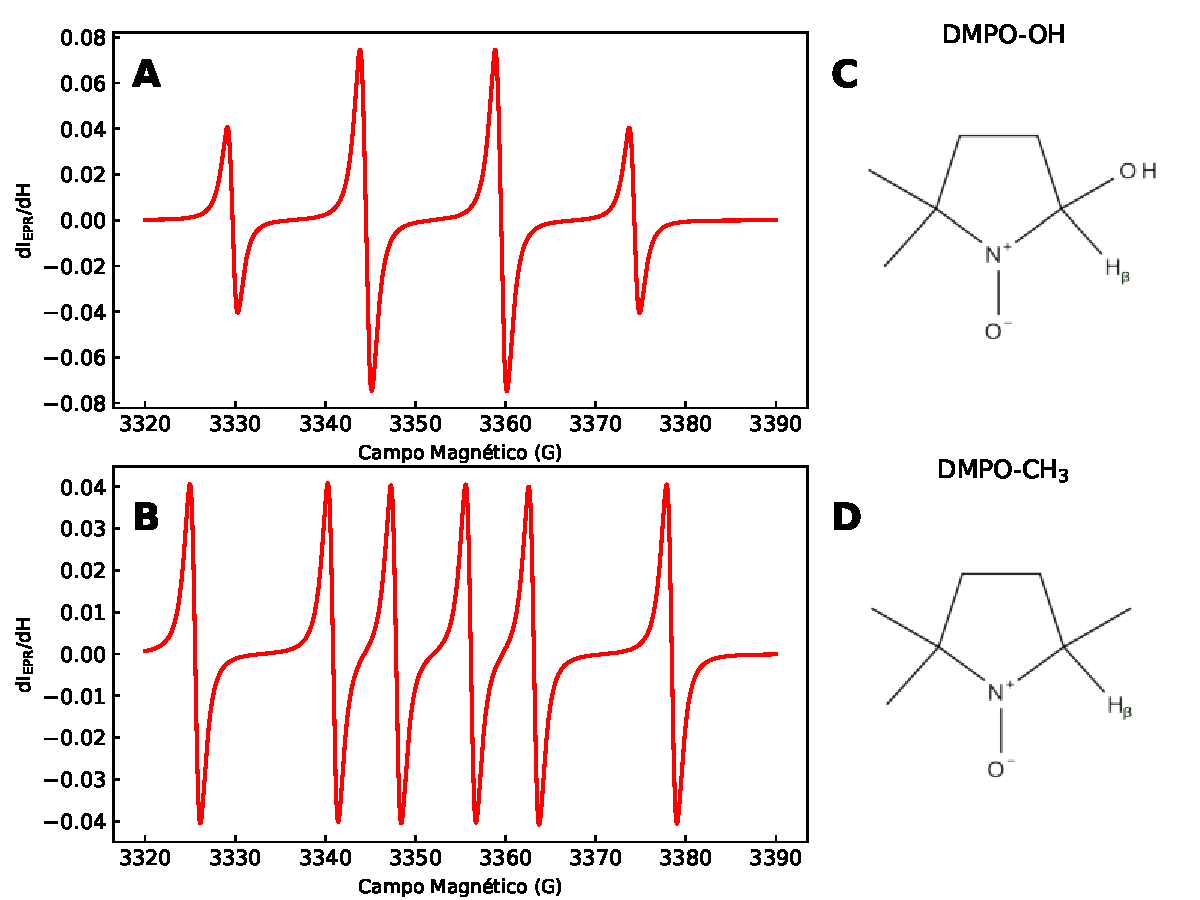
\includegraphics[width=0.95\linewidth]{simulacion.pdf}
    \caption{\centering  A y B muestran la simulación de los espectros esperados para los aductos DMPO-OH y DMPO-CH$_3$ respectivamente en base a las constantes hiperfinas tabuladas por el NIH \cite{nih}. C y D muestran un esquema de la molécula correspondiente a los aductos DMPO-OH y DMPO-CH$_3$ respectivamente.}
    \label{fig:simulacion}
\end{figure}

Para ambos aductos, las constantes de interacción hiperfina se encuentran estandarizadas por el NIH de Estados Unidos (National Institute of Envoirmental Health Sciences) \cite{nih}. Los valores de las constantes hiperfinas tabulados por el NIH para el aducto DMPO-OH son $a_N = 14.9$ G y $a_H = 14.9$ G, mientras que para el aducto DMPO-CH$_3$ son $a_N = 16.1$ G y $a_H = 23.3$ G. Por lo tanto, en base a los valores de referencia del NIH, se propone un modelo para los aductos formados donde el acople hiperfino se da entre el electrón despareado del oxígeno y el espín nuclear del nitrógeno ($I_N = 1$) y el espín nuclear del hidrógeno $H_\beta$ ($I_H=1/2$). Entonces, al aplicar el campo magnético estático $\mathbf{B_0} = B_0 \hat{z}$, según la Ec. (\ref*{ec:Hfinalfinal}), el hamiltoniano que describe estas interacciones es 
\begin{equation}
    \mathcal{H} = g \mu_B B_0 S_z + A_N ~ S_z I_{N,z} + A_H ~ S I_{H,z}.
    \label{ec:HDMSO}
\end{equation}

Para escribir los autoestados de este sistema se necesitan los números cuánticos $M$, $m_N$ y $m_H$. Debido a las aproximaciones mencionadas anteriormente, este hamiltoniano es diagonal en la base de estados $|M,m_N,m_H \rangle$ 
\begin{align}
    \mathcal{H} |M ,m_N, m_H \rangle = &g \mu_B B_0 |M ,m_N, m_H \rangle + \nonumber \\
    &A_N S I_N |M ,m_N, m_H \rangle + \nonumber \\
    &A_H S I_H |M ,m_N, m_H  \rangle
    \label{ec:hamiltoniano_DMPOOH}
\end{align}
y las autoenergías del sistema, es decir los términos diagonales del hamiltoniano son
\begin{equation}
    E_{M, m_N, m_H} = M g \mu_B B_0 + A_N M m_N +  A_H M m_H 
    \label{ec:energiasDMPO}
\end{equation}
donde $M = -1/2, 1/2$, $m_N=-1,0,1$ y $m_H=-1/2,1/2$.

Finalmente, de la condición de resonancia $E_{M, m_N, m_H} = \hbar \omega_{if}$, se determinan los 6 campos de resonancia $B_{0,R}$ para un aducto con las interacciones propuestas
\begin{equation}
B_{0,R} = \frac{\hbar\omega_{if}}{g \mu_B} -  M m_N a_N - M m_H a_H,    
\label{ec:campos}
\end{equation}
donde $a_N = \frac{A_N}{g \mu_B}$ y $a_H = \frac{A_H}{g\mu_B}$.

En la Fig. \ref*{fig:spliteo} se muestran, para valores genéricos de $a_N$ y $a_H$, los niveles de energía dados por la Ec. (\ref*{ec:energiasDMPO}) y las correspondientes transiciones energéticas dadas por las Ecs. (\ref*{ec:reglas}). En base a la Ec. (\ref*{ec:energiasDMPO}) para los niveles de energía y de las constantes hiperfinas tabuladas por el NIH para cada aducto formado, se simularon los espectros EPR como se muestra en las Figs. \ref*{fig:simulacion}A y \ref*{fig:simulacion}B. Para DMPO-OH se esperan ver 4 líneas en relación 1:2:2:1 mientras que para el DMPO-CH$_3$ se esperan ver 6 líneas en relación 1:1:1:1:1:1.

\begin{figure}[ht]
    \centering
    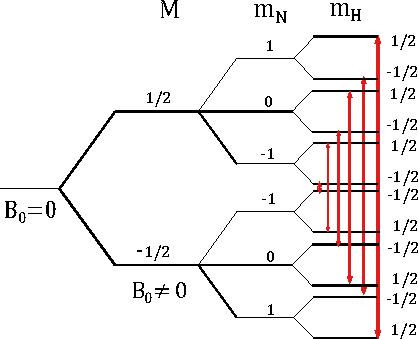
\includegraphics[width=0.675\linewidth]{spliteo.pdf}
    \caption{\centering Espectro de energías para el hamiltoniano $ \mathcal{H} = g \mu_B S_z + A_N S_z I_{Nz} + A_H S_z I_{Hz}$ que modela las interacciones principales del electrón desapareado en la molécula de DMPO. Además, se muestran las posibles transiciones energéticas dadas por las reglas de selección $|\Delta M| = 1$ y $\Delta m = 0$.}
    \label{fig:spliteo}
\end{figure}


\section{Desarrollo experimental}
\subsection{Medición del espectro EPR}
Los experimentos se llevaron a cabo en un espectrómetro Bruker ELEXSYS II E500, equipado con una cavidad rectangular de banda X (9.5 GHz). Se prepararon las nanopartículas con el DMPO disuelto en agua, se agregó H$_2$O$_2$ y se tomó este momento como el tiempo inicial $t=0$. El pH de la muestra era de 5. Se midieron  espectros EPR a los 10 y 40 minutos de añadir el H$_2$O$_2$.

\subsection{Analisis de datos}
Con el objetivo de caracterizar el o los aductos de DMPO formados se ajustó el espectro EPR con una superposición de 6 curvas por aducto correspondientes a derivadas de funciones Lorentzianas \cite{bales_epr_2009}, cada una centrada en el campo de resonancia prescripto por la Ec. (\ref*{ec:campos}). Como se puede ver en dicha expersión, los campos de transición $B_{0,R}$ se calculan a partir de $g$ y de las constantes hiperfinas $a_N$ y $a_H$. Para cada aducto formado se obtuvieron como parámetro de ajuste la intensidad, el ancho de linea, $g$ y las constantes hiperfinas correspondientes. 

\section{Resultados y Discusión}

La Fig. 3A muestra el espectro medido a los 10 minutos. En primer lugar, se observa un conjunto de 3 líneas simbolizadas con (*) que no corresponden a los radicales esperados. En trabajos anteriores \cite{maldonado_actividad_nodate} se identificó esto como un radical debido a configuraciones de la molécula de DMPO y que interacciona solo con el núcleo de nitrógeno por lo que el espectro tiene 3 líneas. Por lo tanto, se ajustó considerando la interacción del radical con el núcleo del nitrógeno junto con las interacciones debido al radical oxhidrilo. De dicho ajuste se obtuvieron las constantes de acoplamiento hiperfino para el oxhidrilo $a_N = (15.00 \pm 0.05)$ G, $a_H =  (14.64 \pm 0.05)$ G, valores que no discrepan de los tabulados por el NIH para el aducto de DMPO con el radical $\cdot$OH. Para el radical del DMPO se obtuvo $a_N = (14.77 \pm 0.05)$ G. Esto es consistente con observaciones \cite{maldonado_actividad_nodate} anteriores donde también se detecto una presencia predominante de radicales oxhidrilo a estos tiempos. 


Por otro lado, la Fig. 3B muestra el espectro medido a los 40 minutos de añadir el H$_2$O$_2$, aquí nuevamente se detecta la presencia predominante de radical oxhidrilo, la presencia del radical de DMPO y además se observa un nuevo conjunto de lineas adicionales (indicadas con \^{}) de muy baja intensidad por lo que se ajustó suponiendo la presencia  del oxhidrilo junto con el radical metilo cuyo hamiltoniano también es de la forma (\ref*{ec:HDMSO}). El ajuste resultó satisfactorio y los resultados de las constantes hiperfinas para el radical oxhidrilo fueron $a_N = (15.01 \pm 0.05)$ G y $a_H = (14.63 \pm 0.05)$ G, valores que no discrepan de los obtenidos en el espectro tomado a 10 minutos lo cual indica que se trata de las mismas especies. Para el radical metilo, $a_N = (15.30 \pm 0.06)$ G y $a_H = (22.35 \pm 0.09)$ G valores que coinciden con lo reportado para dicho radical \cite{maldonado_actividad_nodate}. Para el radical del DMPO se obtuvo $a_N = (14.8 \pm 0.1)$ G. 

\begin{figure}[ht]
    \centering
    
    \begin{subfigure}
      \centering
      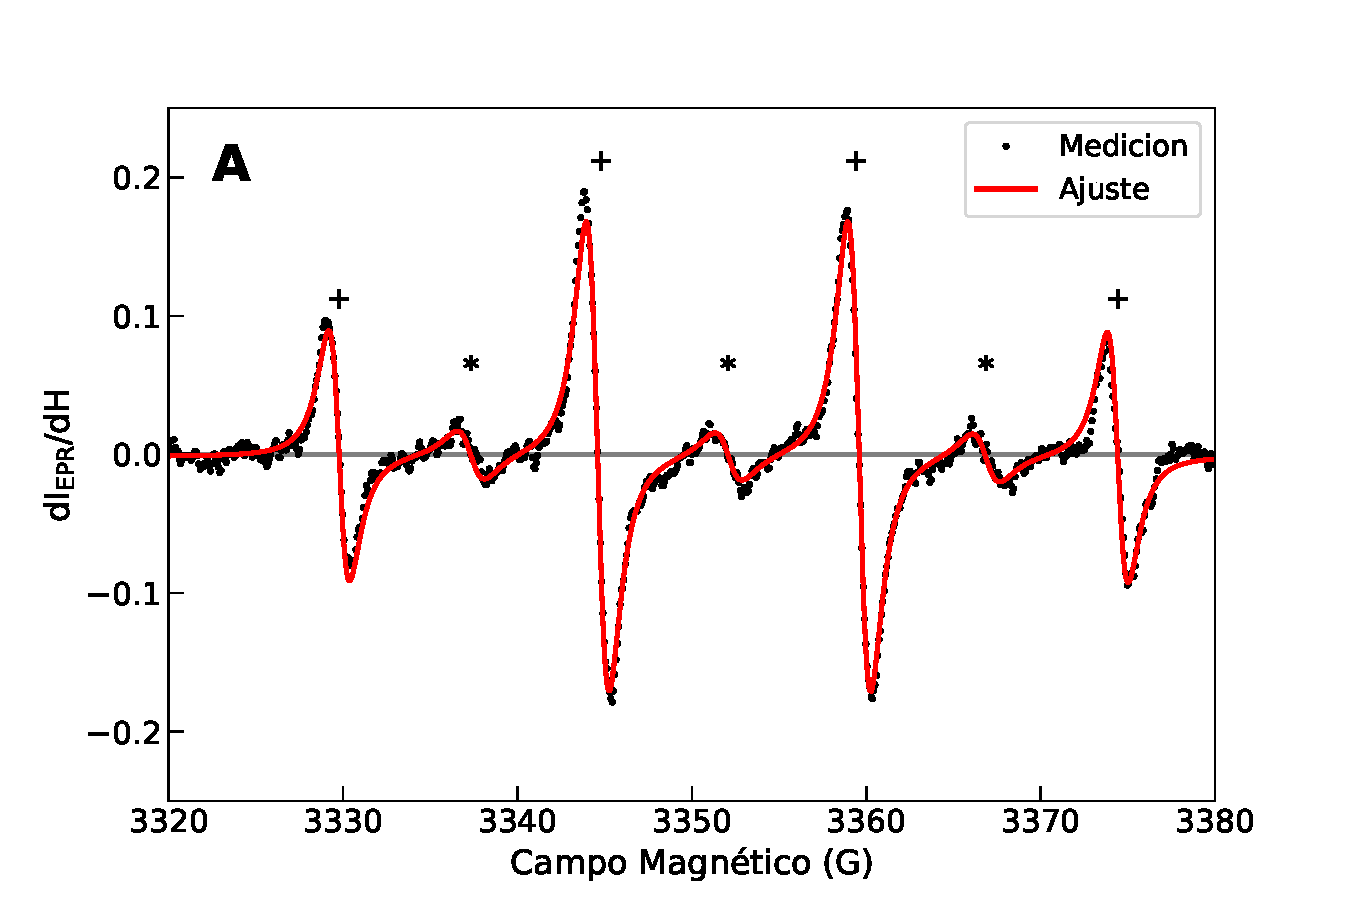
\includegraphics[width=0.95\linewidth]{ajuste_un_radical_lorentzian_10min.pdf}
    \end{subfigure}
    
    \vspace{0.1cm} % Espacio vertical entre las subfiguras
    
    \begin{subfigure}
      \centering
      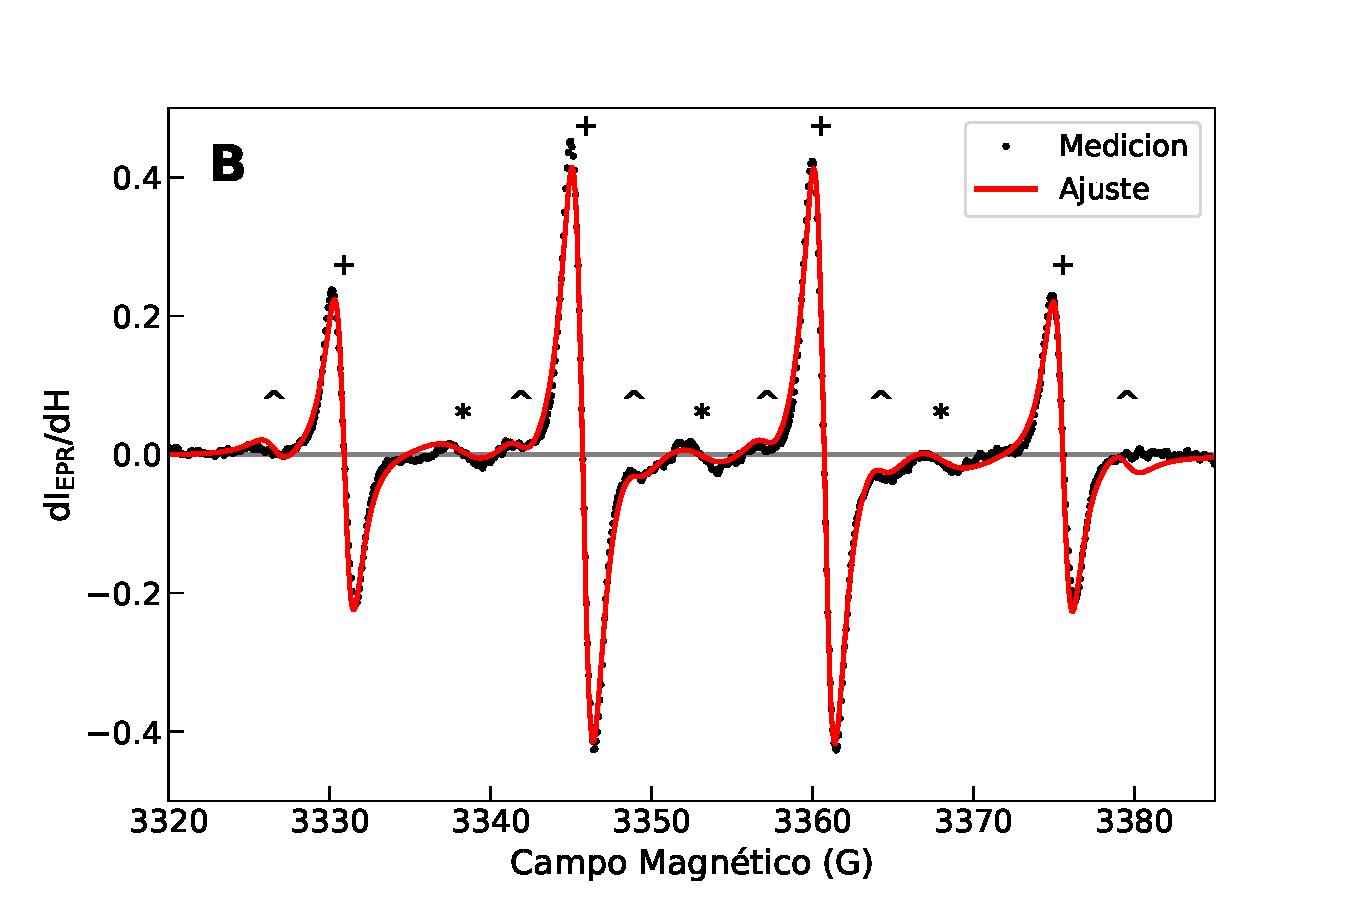
\includegraphics[width=0.95\linewidth]{ajuste_dos_radicales_lorentzian_40min.pdf}
      \label{fig:espectro}
    \end{subfigure}
    
    \caption{\centering Espectro EPR de la muestra de nanopartículas a 10 minutos de añadir H$_2$O$_2$ (A) y a 40 minutos (B). La curva negra corresponde a los datos experimentales y la curva roja es la simulación a partir de los resultados del ajuste. Se marcan las lineas de los grupos radicales $\cdot$OH ($+$), $\cdot$CH$_3$ (\^{}) y el radical debido al DMPO (*).}
  \end{figure}

Los modelos de interacción propuestos resultaron correctos para describir las interacciones presentes dado que se pudieron ajustar bien las lineas presentes en ambos espectros. Además estos resultados fueron consistentes con trabajos anteriores de muestras muy similares.

\section{Conclusiones}

Se estudió la capacidad de promover la producción de ROS mediante nanopartículas de MnFe$_2$O$_4$ en H$_2$O$_2$ utilizando espectroscopía EPR. Debido al corto tiempo de vida de las ROS se implementó la técnica de \textit{spin trapping} para poder detectar la presencia de los radicales formados. El \textit{spin trap} utilizado fue DMPO. En base a trabajos anteriores, se propuso un hamiltoniano para describir las interacciones presentes en los aductos de DMPO formados. 

Se analizaron mediciones tomadas a 10 y 40 minutos del comienzo de produción de ROS y, comparando con trabajos anteriores y la base de datos del NIH se determinó la presencia de radical oxhidrilo a los 10 minutos, con constantes hiperfinas $a_N = (15.00 \pm 0.05)$ G, $a_H =  (14.64 \pm 0.05)$ G. A los 40 minutos, se detectó la presencia de radicales oxhidrilo, con $a_N = (15.01 \pm 0.05)$ G, $a_H = (14.63 \pm 0.05)$ G y de radicales metilo $a_N = (15.30 \pm 0.06)$ G, $a_H = (22.35 \pm 0.09)$ G. 

El modelo de interacción Zeeman e hiperfina para el aducto de DMPO formado resultó ser adecuado para describir los espectros observados. Los resultados obtenidos muestran la capacidad de la técnica de espectroscopía por EPR + \textit{spin trapping} para caracterizar las especies radicales formadas en el proceso de producción de ROS mediante nanopartículas de MnFe$_2$O$_4$ en presencia de H$_2$O$_2$.



%Regular la producción de ROS o neutralizar sus efectos podría ser un enfoque potencialmente efectivo para prevenir y tratar enfermedades relacionadas con el estrés oxidativo. Al mantener niveles óptimos de ROS, es posible aprovechar sus funciones beneficiosas al tiempo que se minimizan sus efectos perjudiciales. Esta investigación abre posibilidades para desarrollar estrategias innovadoras para el manejo de afecciones relacionadas con el estrés oxidativo . 

%La espectroscopía por resonancia paramagnética electrónica (EPR) es una técnica que consiste en desdoblar los niveles de energía electrónicos de una muestra paramagnética mediante un campo magnético estático $\mathbf{B_0}$ e inducir transiciones entre los niveles energéticos a través de la aplicación de un campo magnético oscilante $\mathbf{B_1}$. Para esto, se deben considerar las interacciones entre los espines y el campo magnético estático, y entre los espines electrónicos y nucleares. 

% If in two-column mode, this environment will change to single-column
% format so that long equations can be displayed. Use
% sparingly.
%\begin{widetext}
% put long equation here
%\end{widetext}

% figures should be put into the text as floats.
% Use the graphics or graphicx packages (distributed with LaTeX2e)
% and the \includegraphics macro defined in those packages.
% See the LaTeX Graphics Companion by Michel Goosens, Sebastian Rahtz,
% and Frank Mittelbach for instance.
%
% Here is an example of the general form of a figure:
% Fill in the caption in the braces of the \caption{} command. Put the label
% that you will use with \ref{} command in the braces of the \label{} command.
% Use the figure* environment if the figure should span across the
% entire page. There is no need to do explicit centering.

% \begin{figure}
% \includegraphics{}%
% \caption{\label{}}
% \end{figure}

% Surround figure environment with turnpage environment for landscape
% figure
% \begin{turnpage}
% \begin{figure}
% \includegraphics{}%
% \caption{\label{}}
% \end{figure}
% \end{turnpage}

% tables should appear as floats within the text
%
% Here is an example of the general form of a table:
% Fill in the caption in the braces of the \caption{} command. Put the label
% that you will use with \ref{} command in the braces of the \label{} command.
% Insert the column specifiers (l, r, c, d, etc.) in the empty braces of the
% \begin{tabular}{} command.
% The ruledtabular enviroment adds doubled rules to table and sets a
% reasonable default table settings.
% Use the table* environment to get a full-width table in two-column
% Add \usepackage{longtable} and the longtable (or longtable*}
% environment for nicely formatted long tables. Or use the the [H]
% placement option to break a long table (with less control than 
% in longtable).
% \begin{table}%[H] add [H] placement to break table across pages
% \caption{\label{}}
% \begin{ruledtabular}
% \begin{tabular}{}
% Lines of table here ending with \\
% \end{tabular}
% \end{ruledtabular}
% \end{table}

% Surround table environment with turnpage environment for landscape
% table
% \begin{turnpage}
% \begin{table}
% \caption{\label{}}
% \begin{ruledtabular}
% \begin{tabular}{}
% \end{tabular}
% \end{ruledtabular}
% \end{table}
% \end{turnpage}

% Specify following sections are appendices. Use \appendix* if there
% only one appendix.
%\appendix

% If you have acknowledgments, this puts in the proper section head.

% Create the reference section using BibTeX:
\subsection*{Agradecimientos} % Título personalizado para los agradecimientos
Se agradece al Dr. Teobaldo Torres por proveer las mediciones analizadas en este trabajo
    
\bibliography{trabajo_final.bib}


\end{document}
%
% ****** End of file apstemplate.tex ******
